\chapter{Introduction}

The basic function of a Laptop stand is to support the laptop in different postures. We tried to achieve the same through our Smart Laptop stand. The unique feature of our laptop stand is that it is made of natural materials. Our Laptop stand is made of bamboo and cane. Legs are telescopic and are made of bamboo, while the base or frame part is weaved using cane strips. Different techniques of machining are employed to make telescopic legs, which cater to height adjustment. Base part is made to weave by an artisan, which provides different angles of inclination. Friction pads are also provided to prevent laptop from sliding at any angle of inclination. Techniques employed are of basic carpentry and also artisan work with natural materials, hence this stand can be referred to as a product of cottage industry. 

\section{Problem Statement}

A stand, made of natural materials, which helps the user to interact with laptop in different postures comfortably.

\section{Background}

Nowadays, employees in majority of companies and students in educational institutions prefer laptops, so that they can carry it around and do their work wherever they wish to do. While using a desktop confines us to a sitting posture, usage of laptop gives us additional freedom regarding postures. This freedom costs us fatigue to our body. Efforts are made by an individual to remain in comfortable postures by supporting laptop on their body. Health advisories advise not to work with laptop by supporting them on their thighs or any other body parts, because such usage may cause fatal health issues such as infertility. Laptop stands are designed to prevent these harmful health effects and also to address the problems of fatigue.  

\chapter{Motivation}

We, as a team, through our experience with laptop usage and based on a survey among our student community, decided to take up on this project, to address fatigue problems. We found that, we are not alone in this area,  because, a good amount of research and development have already been done. Through patent search, we discovered that very effective products are already present in the market. But, we found that, almost all products are made of plastic and its related materials. None of them are degradable after complete usage. Also, there are products made of natural materials, but, less effective in terms of functionality and failed to answer some customer requirements. There have been very novel products in terms of design, but the area of novelty in terms of  material selection has not yet explored completely. Our Aim is to make a laptop stand with natural materials such as bamboo and cane. In this way, this product can be manufactured manually (and with some basic carpentry tools) by artisans who have expertise with wood related materials. In this way, an employment opportunity and hence a way of life can be created among people who work in textile industry.

\section{Material Selection}

At present, materials used to make are plastics and its derivatives. Natural materials are never touched upon. Elegant designs are proposed and manufactured using plastic materials.

\section{Novelty}

Novelty of our product is in material selection. So far, from our patent search, it is found that, natural materials are never used to make laptop stands. Although, there are some stands made of natural materials, but lack Robustness in design. Products made of such materials like bamboo, wood, cane etc., has a decent market share. People buy those products to enhance the aesthetic looks of their homes or work spaces. Manufacturing a laptop stand using such materials also creates employment opportunities among artisans in cottage industries\cite{Pinterest}.

\chapter{Target Customers}

Students are our primary target customers, while any others are secondary. 

\section{Survey}

Motivated by our idea, we took a survey, to find out experiences of our friends, about their interaction with laptop. Following are some of the questions and their results from the survey:
119 Responses were collected

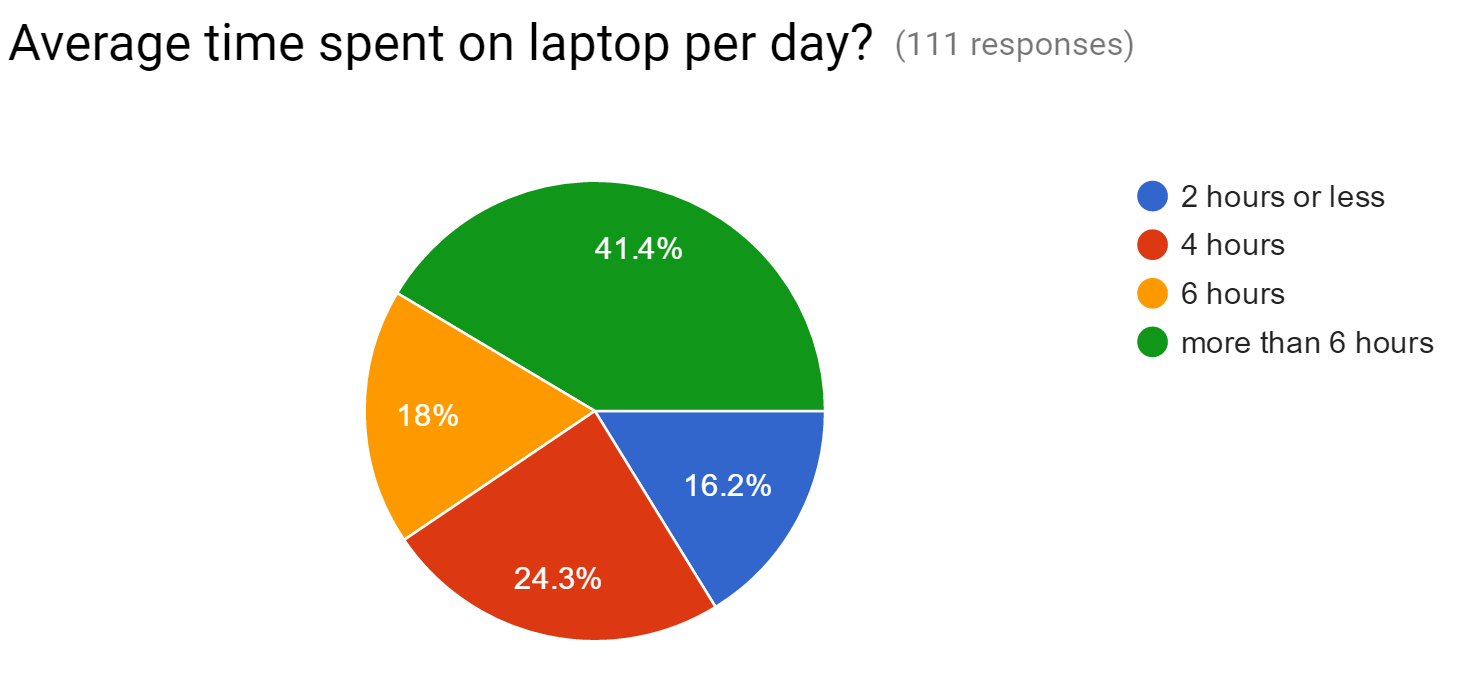
\includegraphics[scale=0.5]{sur1}
\newpage
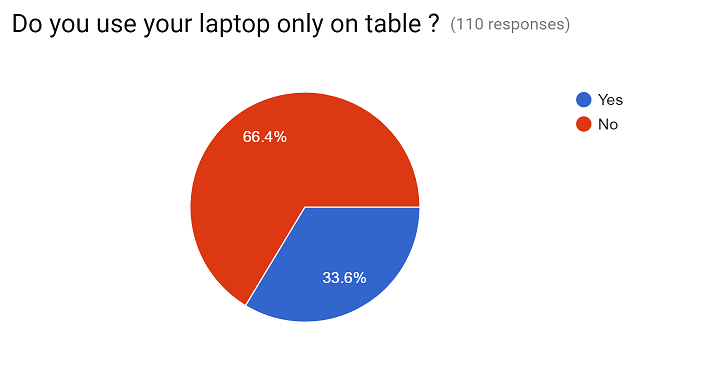
\includegraphics[width=\linewidth]{sur2}
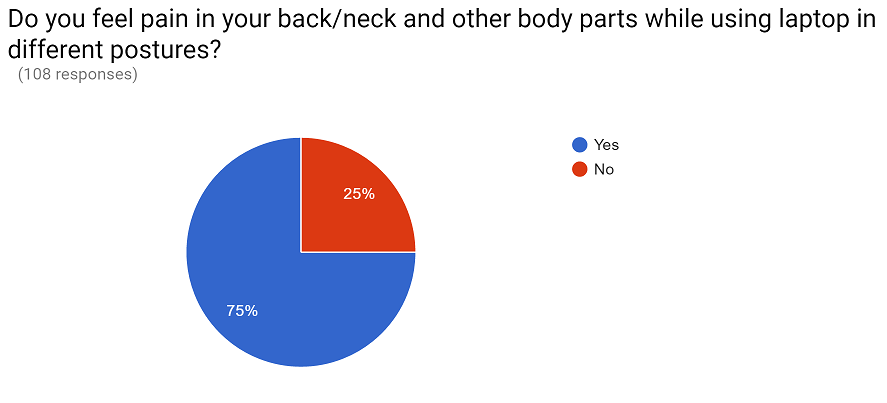
\includegraphics[width=\linewidth]{sur3}
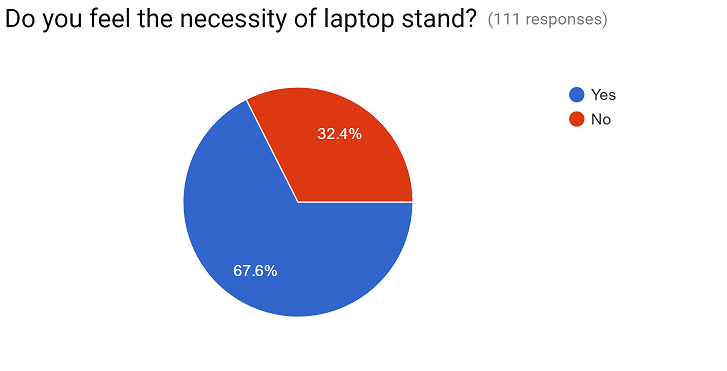
\includegraphics[width=\linewidth]{sur4}
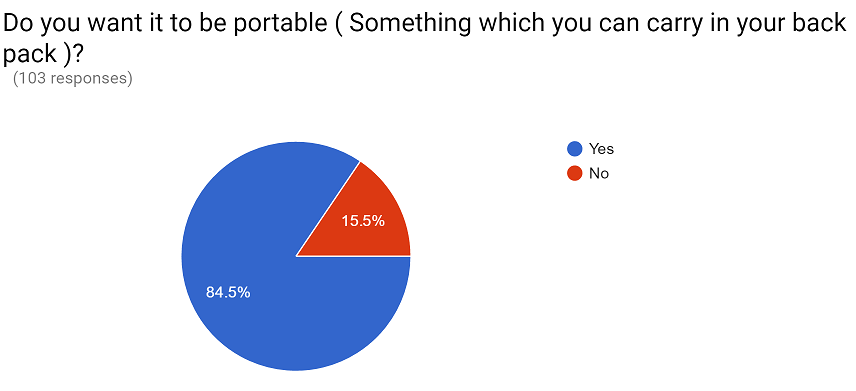
\includegraphics[width=\linewidth]{sur5}
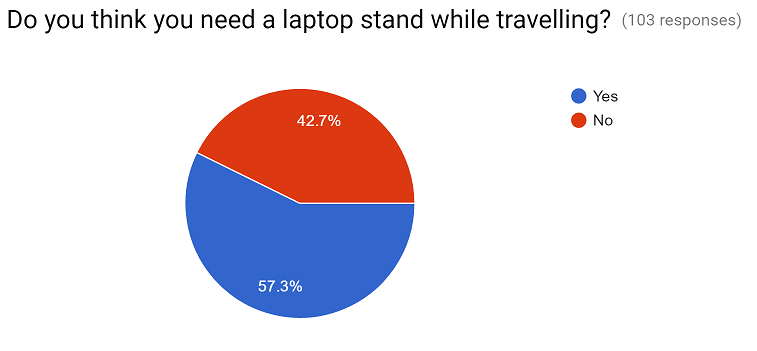
\includegraphics[width=\linewidth]{sur6}
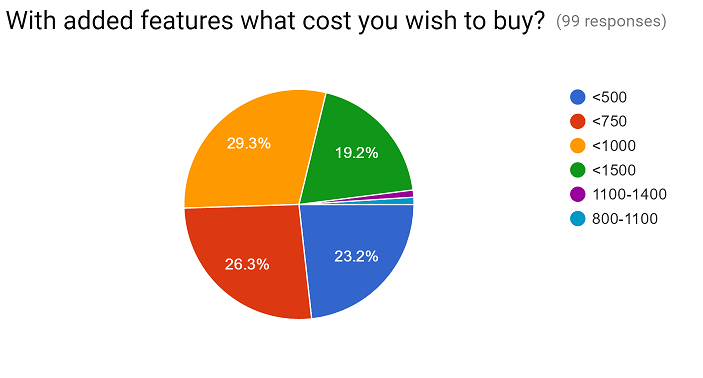
\includegraphics[width=\linewidth]{sur7}

Also, a survey is taken among student community, about the usage of laptops in frequently seated or rested postures. 


\section{Conclusion from Survey}

From the survey it is also found that, the range of cost is in between 750-1000 rupees.

\chapter{Challenges}

There are wide range of  laptop stands in Market. Most of them in one way or the other, cater to the different needs of customers. Always, there exists a tradeoff between functionality and cost. Most of the stands are from foreign market, which are advertised for Macbook. In Indian market, the stands which are available do not cater to all customer requirements. Stands, made of natural materials lack robustness in design, and also they do not provide all the requirements which plastic stands are providing.  


\section{Cons of Existing Products from Customer Reviews}

Reviews from websites like Flipkart, Amazon, ebay are analysed and some common cons are picked. They are as follows:\cite{amazon_site}

\begin{itemize}
 \item Delicate parts
 \item Cheap material used for manufacturing the product
 \item Legs not bearing enough loads and are deforming easily
 \item No proper locking for legs
 \item Reliability issues like strength, type of usage
 \item Not so user-friendly, like cumbersome to adjust height.
 \item Difficulty for all the legs to be in the same plane which leads to wobbling.
 \end{itemize}
 
 \section{Customer Requirements}
 
 Through the survey and based on reviews about the present laptop stands in the websites as mentioned earlier, certain general customer requirements are observed as follows:
 
 \begin{itemize}
 \item Less weight ( since no one wants to carry an extra 2 kg )
 \item Portable
 \item Easy to use
 \item Low cost
 \item Ability to support different postures
 \end{itemize}

\chapter{Concept Selection}

From market analysis, we observed that, present designs made of plastic are robust enough, which the stands made of natural materials lack. Keeping this aspect in mind, we ideated concepts, which might have already been there, but never approached with natural materials. Through the concepts, basic requirements such as height and angle adjustment, are primarily addressed.

\section{Design 1}

Height of the stand can be changed by shifting the position of the rod that is connected to the upper part of the stand and by using the cris-cross mechanism. 

\begin{figure}
  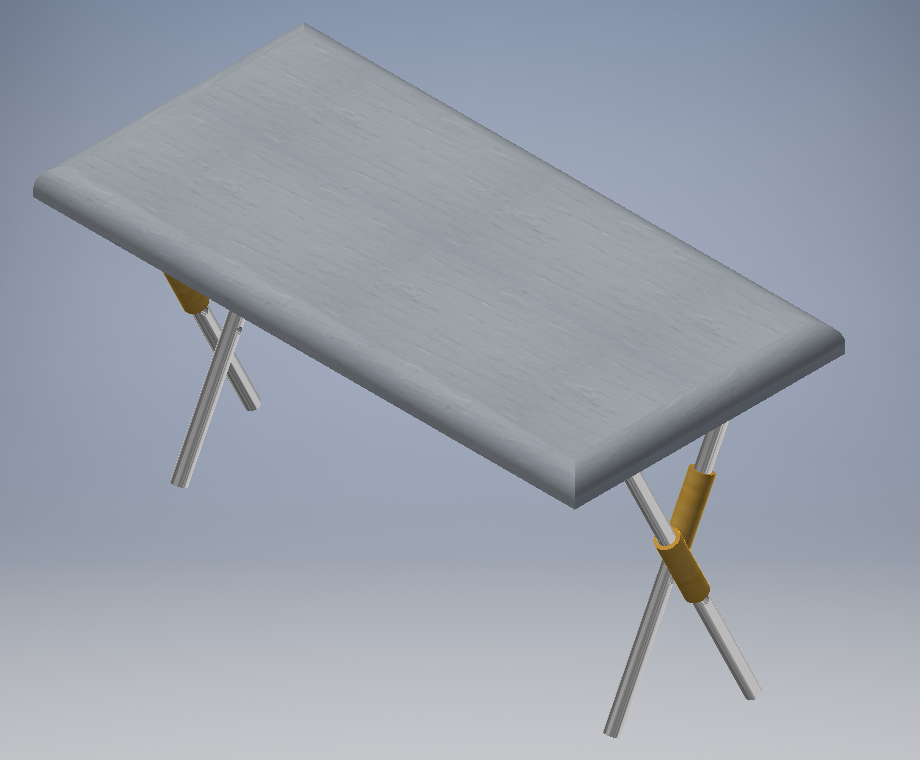
\includegraphics[width=\linewidth]{design1}
  \caption{3-D Model of Design1.}
  \label{fig:Design1}
\end{figure}


\begin{itemize}
 \item Pros
 \begin{enumerate}
	\item Portable
    \item Easy to use
    \item Adjustability
 \end{enumerate}
 \item Cons
 \begin{enumerate}
	\item Lack of Stability
    \item Cannot change the angle
 \end{enumerate}
\end{itemize}



\section{Design 2}

A scissor like mechanism used for height adjustability. A handle is rotated clockwise to lift the scissor mechanism on which the laptop rests\cite{american_manf}.

\begin{figure}
  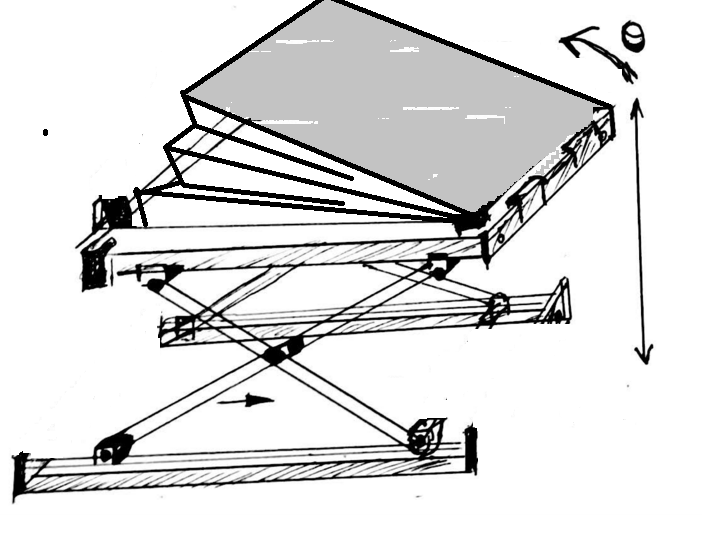
\includegraphics[width=\linewidth]{design2}
  \caption{3-D Model of Design2.}
  \label{fig:Design2}
\end{figure}

\begin{itemize}
 \item Pros
 \begin{enumerate}
	\item Angled sharply towards user and held securely.
    \item Easy to increase or decrease the height of the stand.
    \item It opens and closes easily and this design can hold more weight.
 \end{enumerate}
 \newpage
 \item Cons
 \begin{enumerate}
	\item The mechanism makes the laptop stand heavy.
    \item To adjust the height the laptop should be at the edge of the table.
    \item Occupies more space
 \end{enumerate}
\end{itemize}

\section{Design 3}

A detachable design, where the base is foldable and the legs are telescopic, detachable. Tilt can be varied by adjusting two legs\cite{adj_kbtray}.

\begin{figure}
  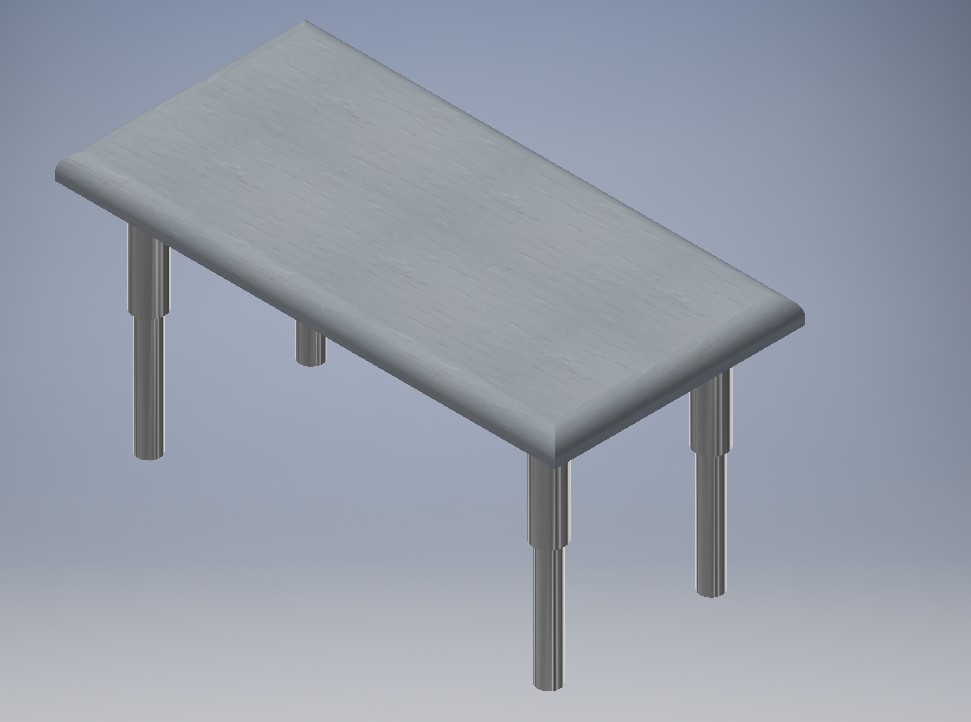
\includegraphics[width=\linewidth]{design3_1}
  \caption{3-D Model of Design3.}
  \label{fig:Design1}
\end{figure}

\begin{figure}
  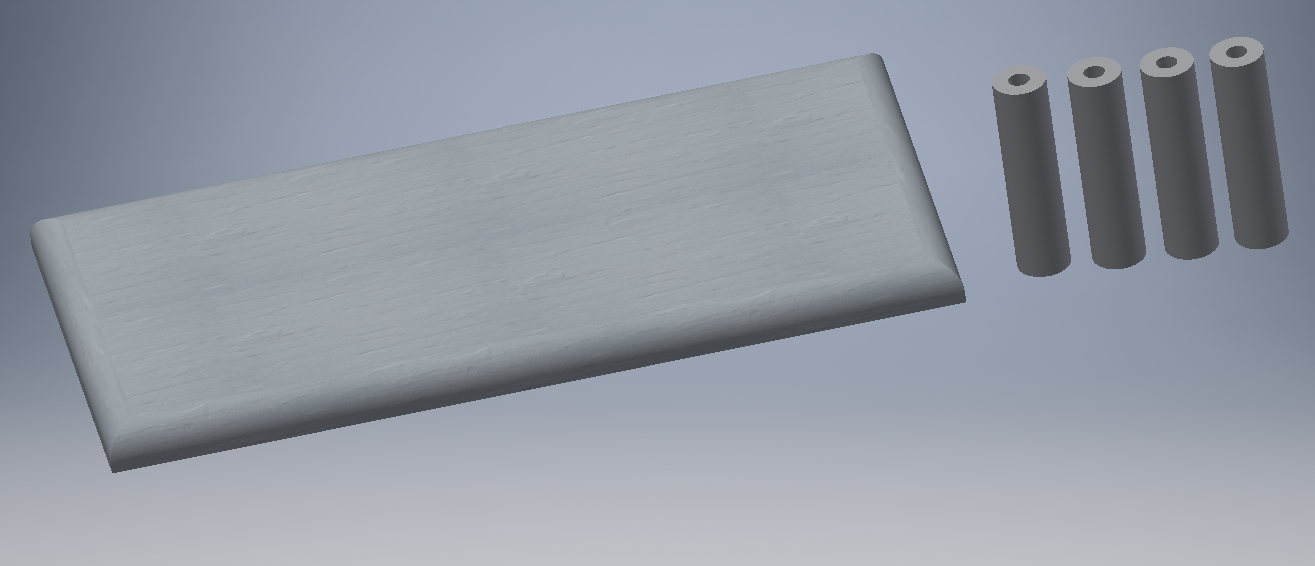
\includegraphics[width=\linewidth]{design3_2}
  \caption{3-D Model of Design3 ( Legs removed ).}
  \label{fig:Design1}
\end{figure}

\begin{itemize}
 \item Pros
 \begin{enumerate}
	\item The legs can be compressed and detached.
    \item The tilt can be changed to any angle.
 \end{enumerate}
 \item Cons
 \begin{enumerate}
	\item Difficult to adjust the legs simultaneously to the same length.
    \item The weight bearing capacity of the leg is limited.
 \end{enumerate}
\end{itemize}

\chapter{Final Design}

\section{Why this concept}

Among the three designs proposed, Design-3 is identified as suitable one to continue with. Certain modifications are done such as, tilt adjustment is done by providing inclinations to the base through leverage.  Design-1 lacks stability, while Design-2 adds more weight than required. Both the concepts lack novelty, and both the designs cannot be manufactured using the proposed raw materials. In Design-3, manufacturing telescopic legs with bamboo adds novelty to the product, hence it is preferred. 

\section{Design Concept}

\begin{itemize}
\item To provide different heights and angles, so that the laptop stand can be used according to one’s convenient posture. 

\item The telescopic legs are cylindrical in shape which are made of bamboo. Each leg has three components. L shaped grooves are made in each component where a bead present in both inner legs slide through it. They cater to three different positions in vertical direction.

\item Base consists of two components joined by hinges. One component consists of horizontal bars, which supports the other component to incline through leverage. This provides base with three different angles of inclination.

\item Legs are detachable and can be attached by tight fitting them to the cylindrical cane beads which are provided to the base. They can be easily compressible to their minimum length and are easy to carry.

\end{itemize}

\section{Specifications and Metrics}

Based on the survey and reviews, certain specifications are decided, and certain metrics are ascertained. They are as follows:

\begin{table}[h!]
  \centering
  \caption{Specifications and Metrics.}
  \label{tab:table1}
  \begin{tabular}{l||l}
  	\hline
  	Specifications & Metrics\\
    \hline
	Weight & less than 2 kg\\
	Portable ( volume ) &1000-2000 cc\\
	Removable legs & 4 (Number of legs)\\
	Stability & location of center of gravity\\
	Height adjustable & 3 different steps\\
	Number of postures & 4\\
	Orientation & 3 different angles\\

  \end{tabular}
\end{table}

Through measurements and based on the availability of raw materials specifications are redefined and modified as follows:

Maximum height required = 42 cm.
\newline
Maximum inclination = 50 degrees.

\begin{table}[h!]
  \centering
  \caption{Features and Metrics.}
  \label{tab:table2}
  \begin{tabular}{l||l}
  	\hline
  	Specifications & Metrics\\
    \hline
	Weight & less than 2 kg\\
	Portable ( volume ) &1000-2000 cc\\
	Removable legs & 4 (Number of legs)\\
	Stability & location of center of gravity\\
	Height adjustable & 3 different steps\\
	Number of postures & 4\\
	Orientation & 3 different angles\\

  \end{tabular}
\end{table}


\chapter{Prototyping}
Following are some steps that are followed while prototyping our product.
\begin{itemize}
	\item Collection of raw materials
	\item Exploring Methods of Manufacturing
	\item Manufacturing of Telescopic legs
	\item Challenges and difficulties in manufacturing
	\item Selection of raw material for base
	\item Procuring of artisan to manufacture base
	\item Weaving of the base part
    \item Joining of base and telescopic legs

\end{itemize}

\section{Raw Material}

The raw material chosen to manufacture telescopic legs is bamboo. It is available in different varieties. Generally long poles of bamboo is used to provide as a support to structures during construction. It’s known for its strength and lesser weight. It comes with natural tapering. Some other properties of bamboo is noted in the table below.

\begin{table}[h!]
  \centering
  \caption{Bamboo properties and Metrics.}
  \label{tab:table3}
  \begin{tabular}{l||l}
  	\hline
  	Properties & Metrics\\
    \hline
	Compressive Strength  & 80 MPa\\
	Density & 0.7 g/cc\\
	Elastic Modulus & 18 GPa\\
	Elongation ( for a particular load ) & 6\\
	Strength to weight ratio & 57 kN-m/kg\\
	Ultimate tensile strength & 40 MPa\\
	Inner to outer diameter ratio & 0.823\\

  \end{tabular}
\end{table}

As noted above, bamboo has high Strength to weight ratio, which makes it as a reliable material for our product. 

\section{Exploring Methods of Manufacturing}

Different sizes of bamboo is bought, which are available in lengths of 10-12 feet. The ratio of inner to outer diameters is smaller than expected and there is a natural tapering. Required lengths and sizes of bamboo pieces are cut  and drilling is done longitudinally, between inner and outer diameters, using drill bits of different sizes. Turning machine is also used to drill holes. Drill bits of smaller diameters such as 2mm, 3mm are used to drill holes through the thickness of the bamboo\cite{bamboo_flute}. 

\section{Manufacturing of Telescopic Legs}

In our product, as mentioned earlier, Telescopic legs are height adjustable. The components of each leg of appropriate lengths are separated from raw bamboo by cutting it using Angle grinder. Each leg consists of three bamboo sticks of appropriate lengths and different diameters. Holes are made longitudinally, that is along the length of each stick, such that the ratio of inner to outer diameters is maintained close to 0.823 and also such that legs of smaller diameter slide through the drilled holes. Making holes means increasing the inner diameter of bamboo sticks, this is called boring, which is done by using Turning Machine. L shaped slots are made in two outermost legs through which a bead (here we used nails as beads) present in two innermost legs slide and lock. The slots are made using angle grinder. A grinding wheel of thickness 3mm is used to grind the slots in horizontal and vertical directions to get L shape.

\section{Raw material for base}

Plywood, Medium Density Fiberboard (MDF), Cane and Bamboo are potential materials for the base. Following are some tables to compare these materials\cite{bamboo_mdf}.

\begin{table}[h!]
  \centering
  \caption{Properties of Plywood and MDF}
  \label{tab:table4}
  \begin{tabular}{l||l}
  	\hline
  	Plywood & MDF\\
    \hline
	Gives natural look   & Better surface finish\\
	Low Density & Ease of machining\\
	Ease of Machining, Economical & Cheaper than plywood\\
	Common thicknesses are 3,4,6,9 and 12mm & Common thicknesses are 3,4,6,9 and 12 mm\\
	Stronger than MDF & Easy to Laminate\\
  \end{tabular}
\end{table}

Both the materials, Plywood and MDF adds extra weight to the laptop stand.

\begin{table}[h!]
  \centering
  \caption{Subjective comparison of Bamboo and cane}
  \label{tab:table5}
  \begin{tabular}{l||l}
  	\hline
  	Attribute & Comparison\\
    \hline    
	Strength & Bamboo is slightly better than cane\\
	Weight & Bamboo is slightly lighter \\
	Cost & Cane is marginally Costlier\\
	Aesthetic appeal & Cane looks aesthetically better\\
	Rigidity & Weaved cane is more rigid than bamboo\\

  \end{tabular}
\end{table}

Bamboo strips when weaved leads to an uneven pattern and do not have much strength. On the other hand, cane strips are easy to weave, they have good tensile strength and an uniform weave surface can be worked out easily. Hence, cane weave is preferred.

\section{Weaving the base part}

Weaving is an art which comes by practice. Hence we preferred an artisan to manufacture the base part for our prototype. A CAD model has been made and appropriate dimensions are explained to the artisan. 
As explained before, the base consists of two components, both of them attached by standard door hinges. Both the components are made by joining (using nails) cane cylindrical rods as the outer rectangular structure. One of the components consists of  horizontal bars, parallel to the length of the rectangular structure, which are spaced at calculated distances, so that they provide as support and also cater to different angles of inclinations. To the other part of the base cane strips are weaved to cover the structure completely. To the back of it two rods are provided as leverage, so that the weaved part lifts and stays at an inclined position on the support provided by other component. 

\section{Joining of base and legs}

Cylindrical beads are made such that the telescopic legs can be snug fitted into them. They are subjected to turning machine, so that their diameters slightly lesser than that of telescopic legs. Sanding sheet is used to reduce the diameters of beads so that they can be provided with snug fit. These beads are nailed into the base, leaving a projection to which legs are attached. The legs are easily removable and stored. 

\section{Provision of Friction Pads}
Friction pads are necessary to prevent laptop from sliding when placed at an inclined posture. To achieve this, rubber material is pasted on a square sheet (also a friction pad) along the four corners of Laptop stand. Erasers are used as rubber material.

\begin{figure}[h]
    \centering
    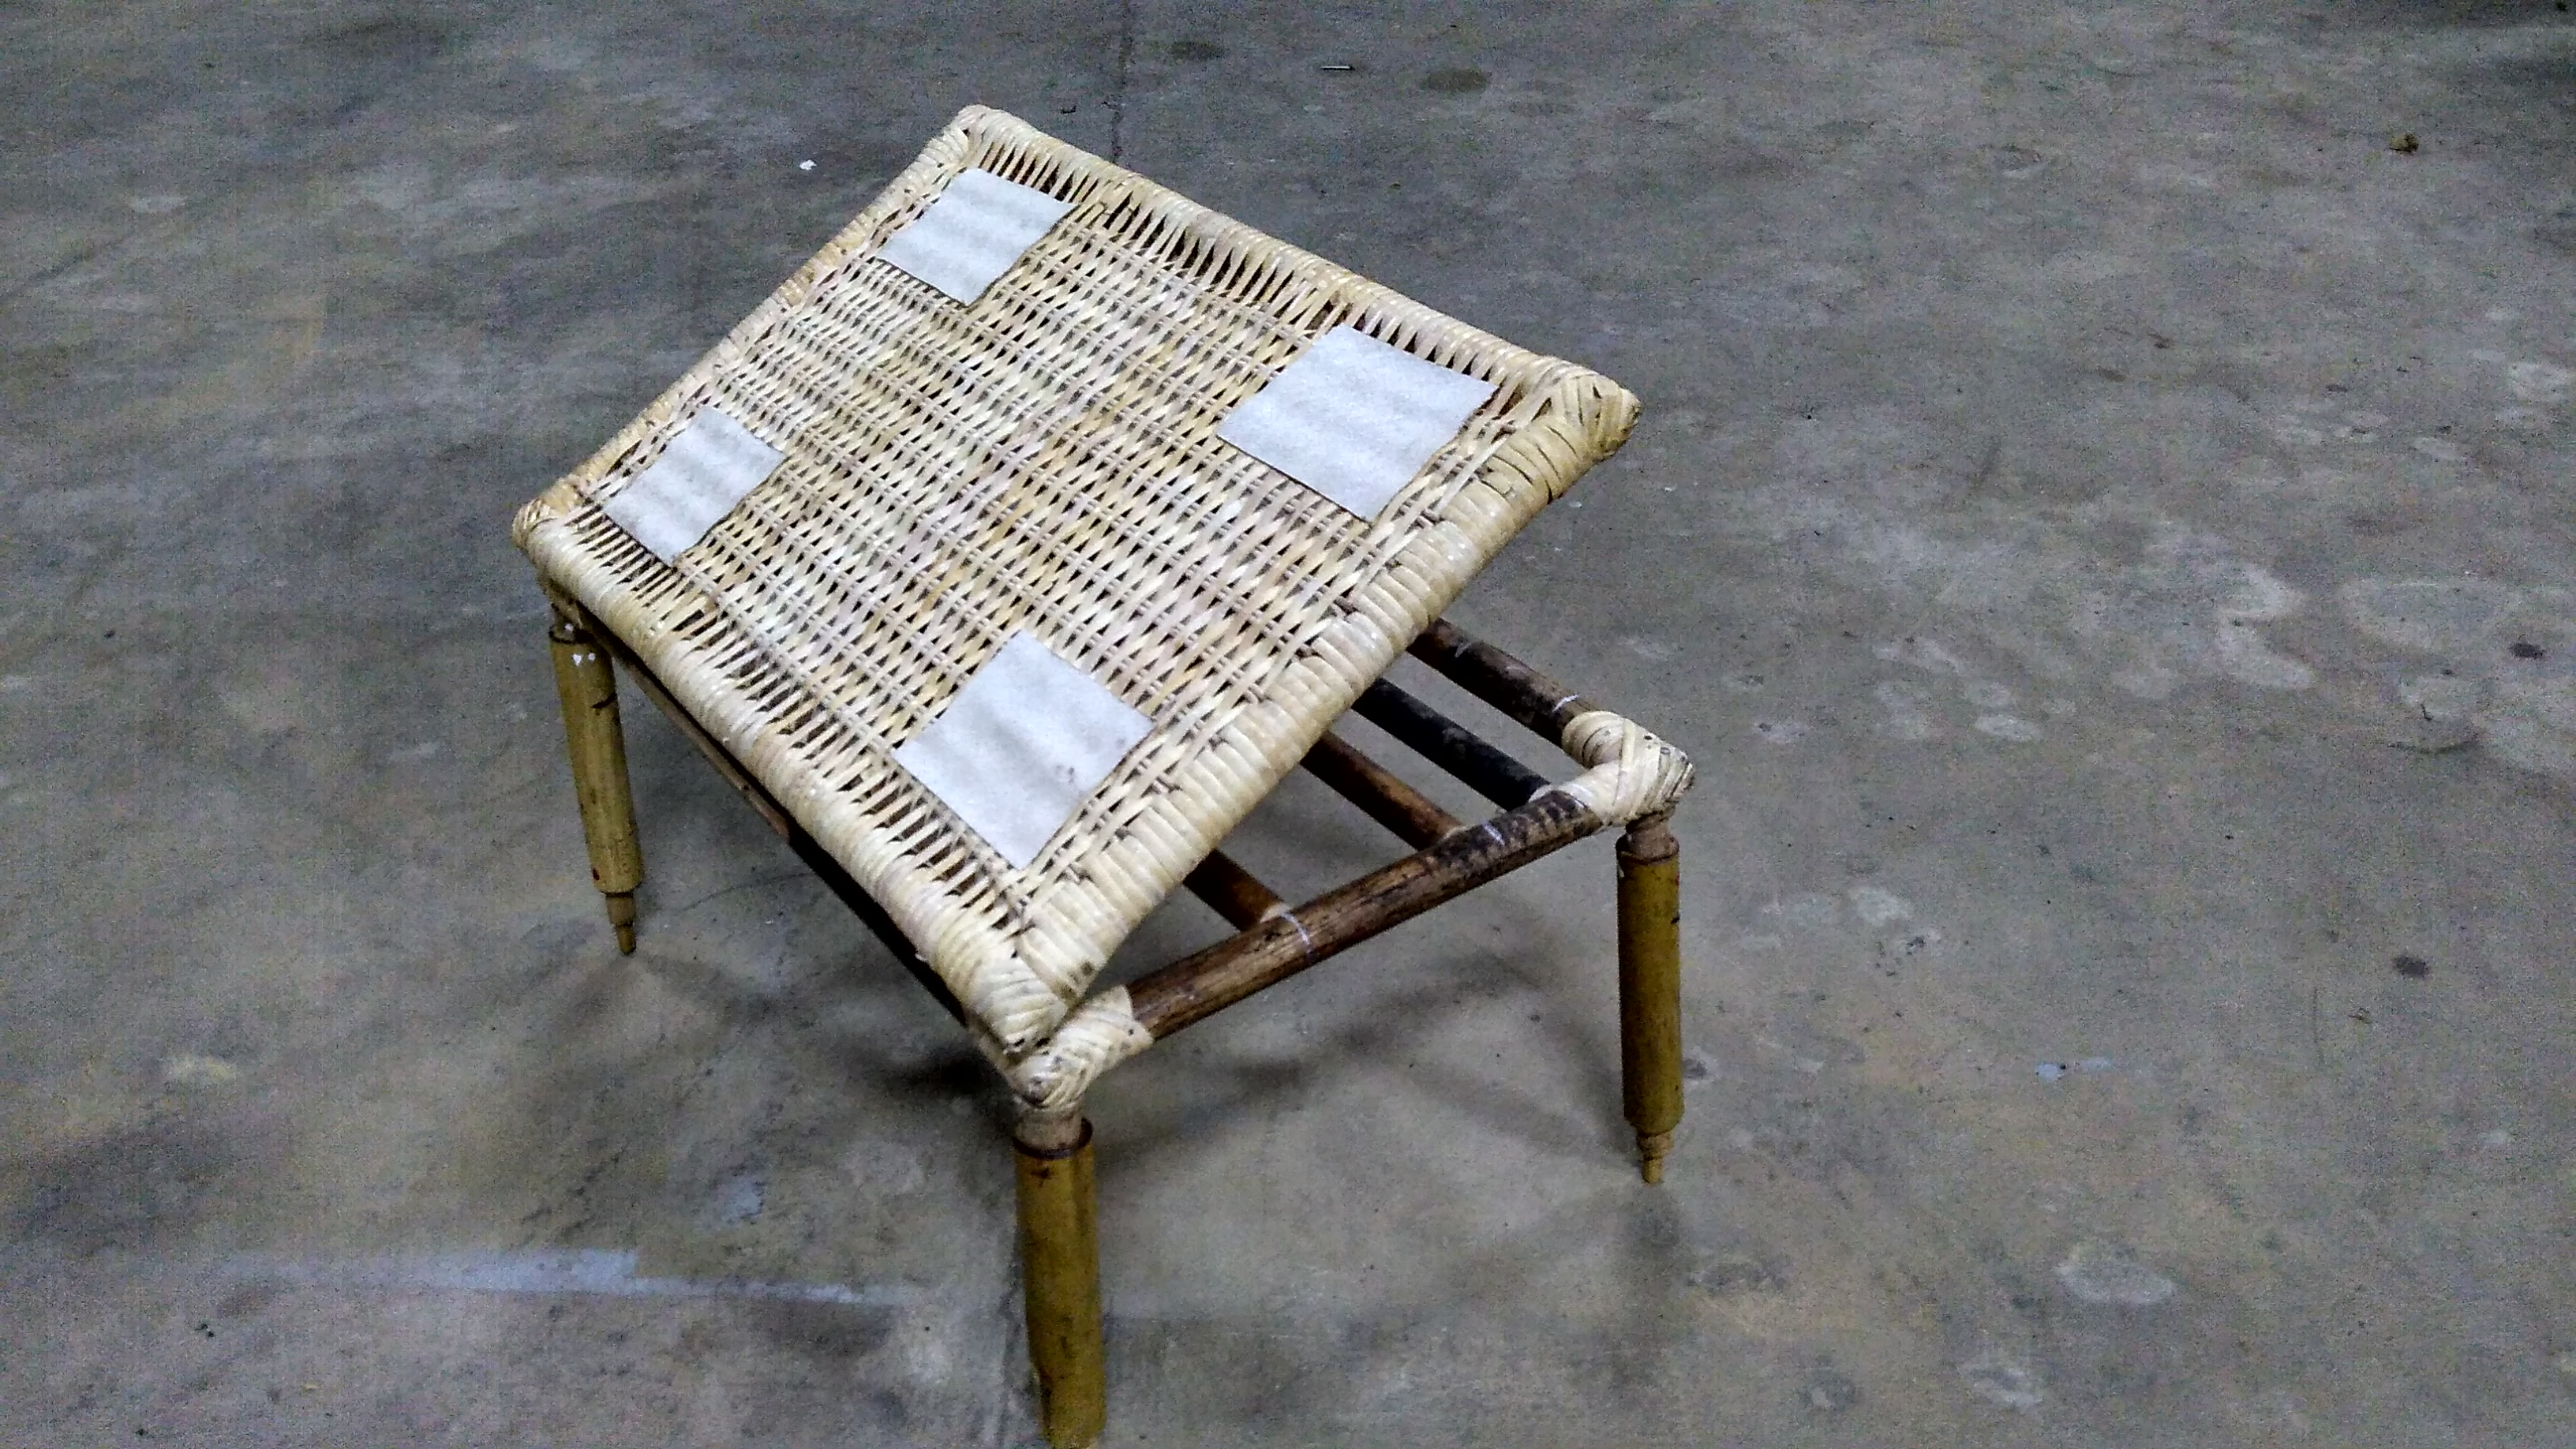
\includegraphics[width=\linewidth]{fi1}
    \caption{Final product ( All legs compressed and table surface oriented at an angle )}
    \label{fig:mesh1}
\end{figure}

\begin{figure}[h]
    \centering
    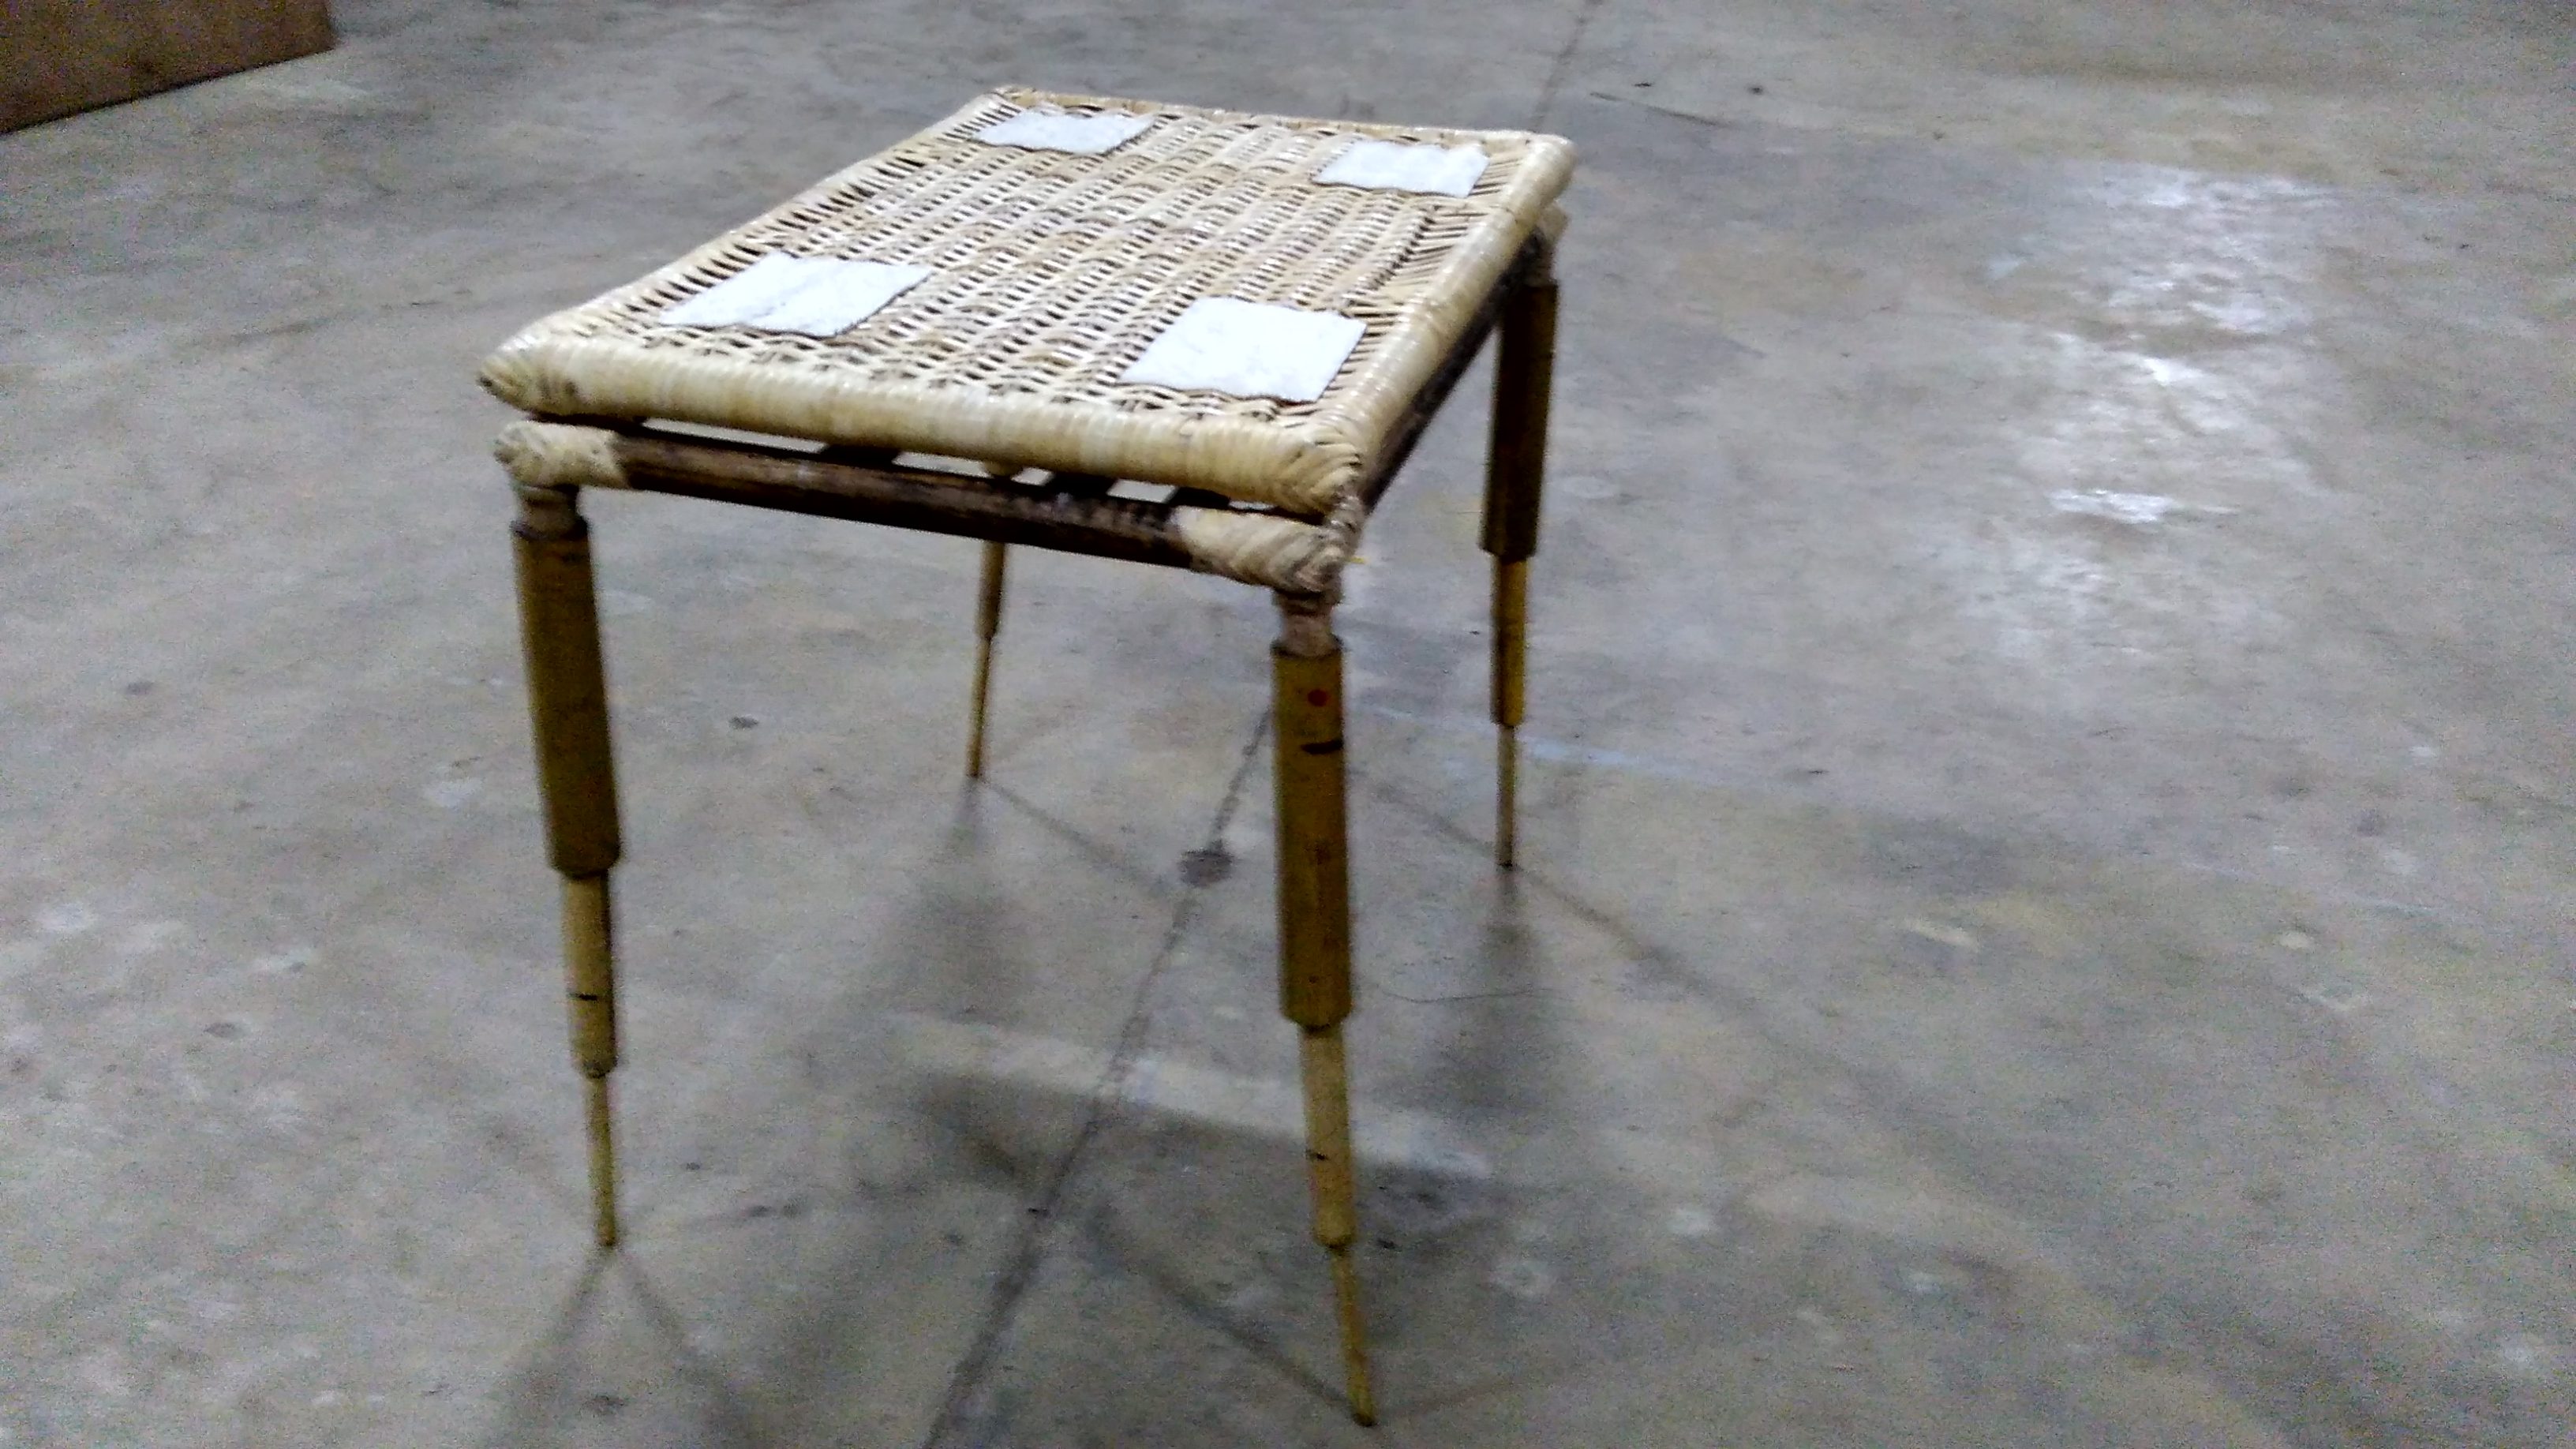
\includegraphics[width=\linewidth]{fi2}
    \caption{Final product ( All legs expanded and table surface oriented horizontally )}
    \label{fig:mesh2}
\end{figure}

\begin{figure}[h]
    \centering
    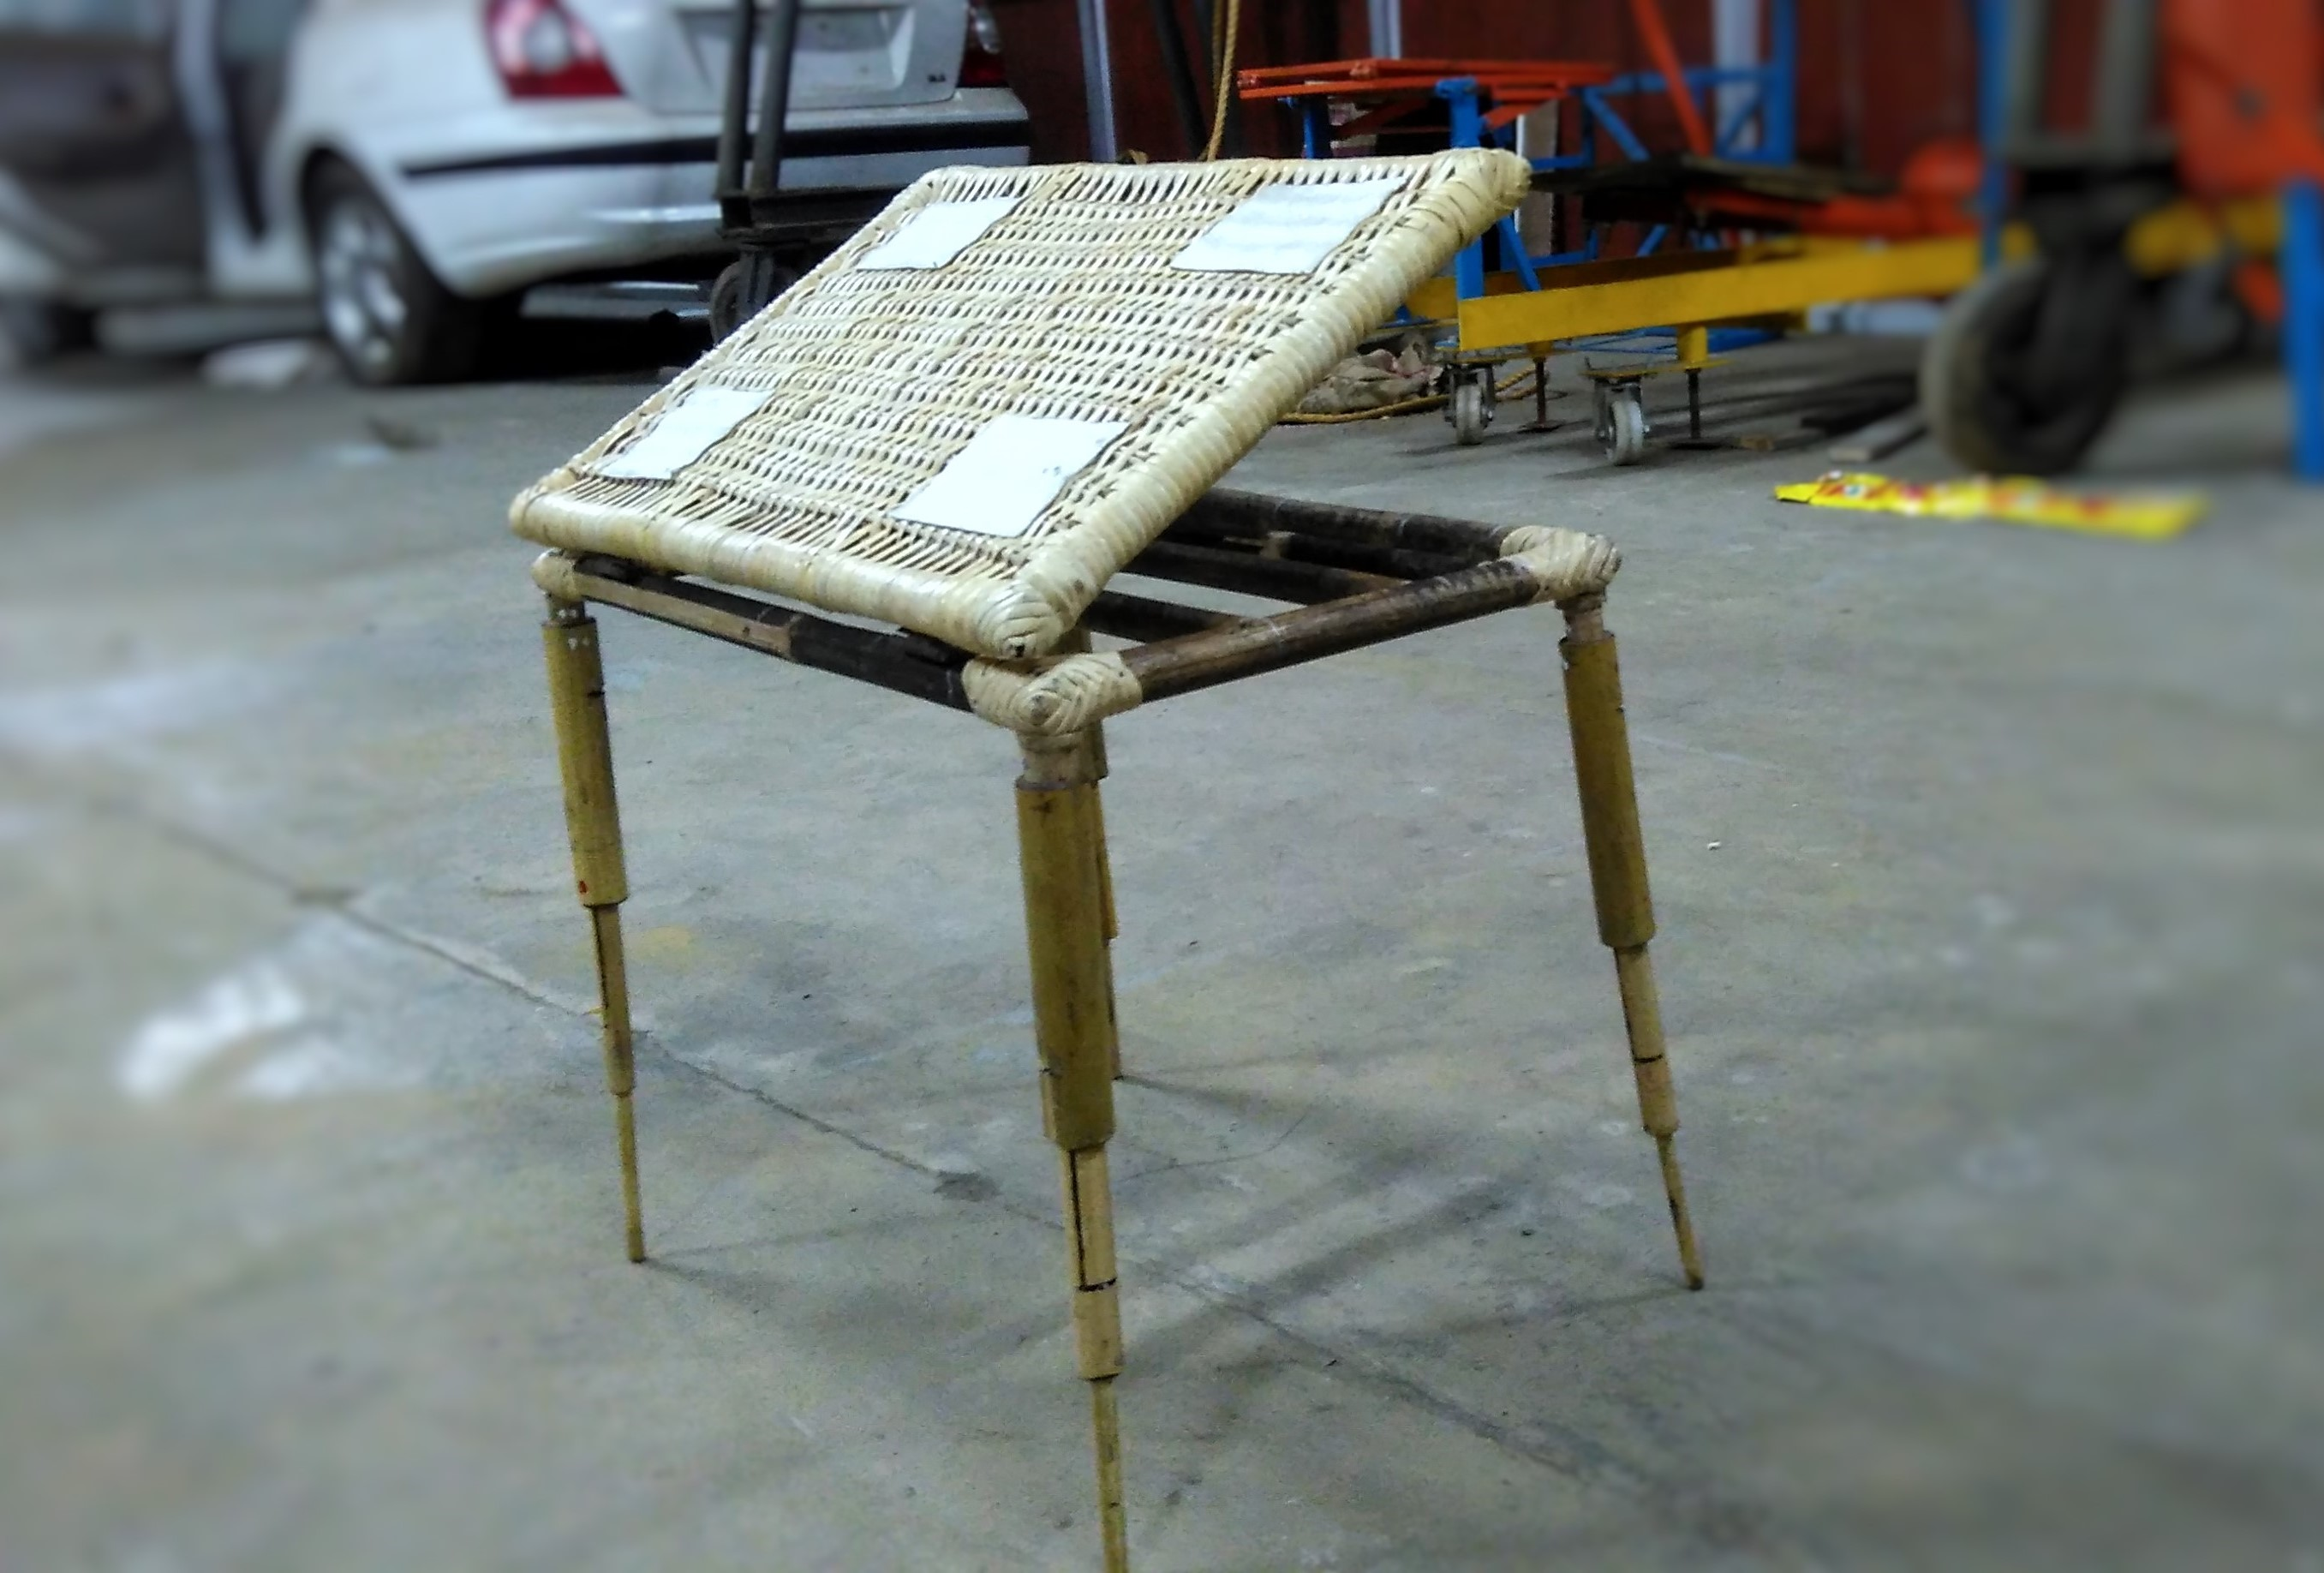
\includegraphics[width=\linewidth]{fi3}
    \caption{Final product ( All legs expanded and table surface oriented at an angle )}
    \label{fig:mesh3}
\end{figure}

\begin{figure}[h]
    \centering
    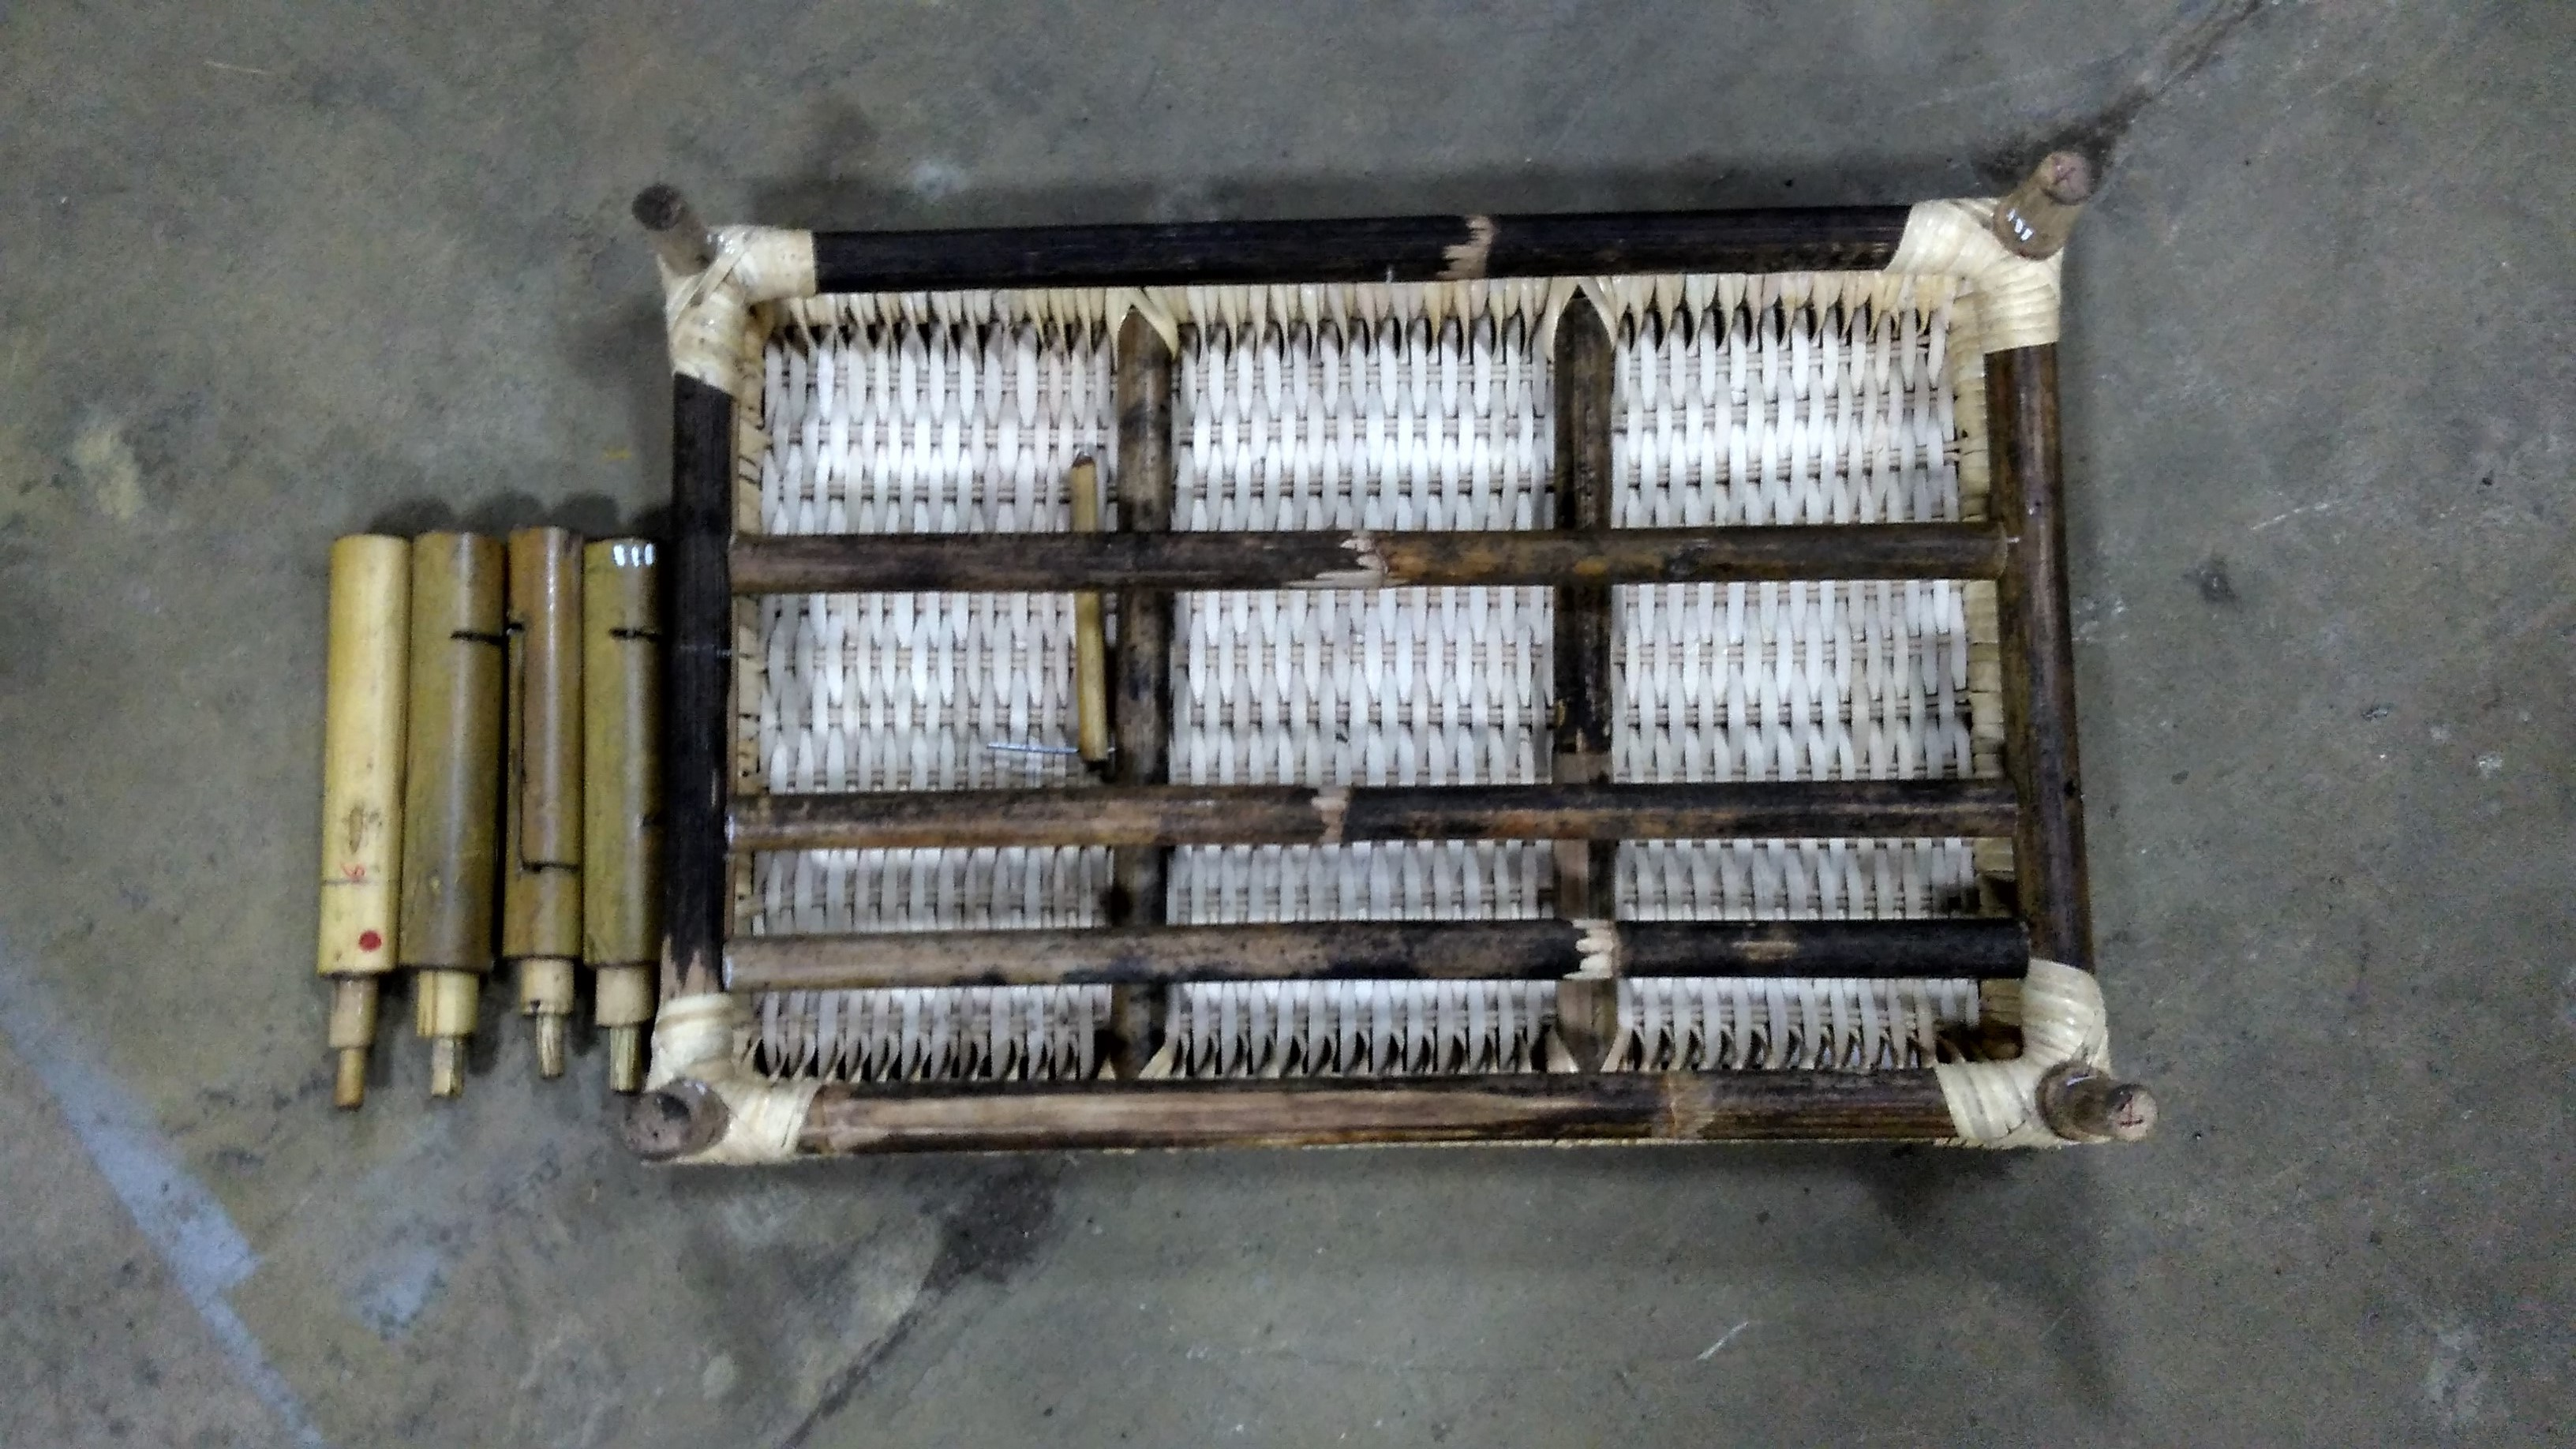
\includegraphics[width=\linewidth]{fi4}
    \caption{Final product ( Table top and all legs removed)}
    \label{fig:mesh4}
\end{figure}


\section{Challenges and difficulties while manufacturing with bamboo}

\begin{itemize}
	\item Working with bamboo created many challenges such as, difficulty in drilling, boring, 		turning and slot cutting. 
	\item Finding the right sizes of bamboo and also manufacturing techniques is a challenge in 	itself. 
	\item Failure of legs due to improper provision of slots or due to cheap quality of bamboo.
	\item Presence of natural tapering in bamboo lead to unnecessary clearance, which made the 	structure wobble.

\end{itemize}

\section{Flaws in design}

\begin{itemize}
\item The design is not completely made of natural materials, due to the presence of components like nails, door hinges, rubber pads. 
\item Absence of friction pads to the legs.
\item Wobbling of the stand

\end{itemize}

\chapter{Conclusion}

\section{Scope of Improvement}

\begin{itemize}
\item Instead of using door hinges for joining components of base, natural weave techniques can also be used.
\item Rubber pads can also be removed and their role can be given to the type of weave, like creating uneven weave surface at the corners might provide sufficient roughness to hold the laptop when it is inclined.
\item Arranging rubber stoppers to the legs so that wobbling can be prevented to some extent.
\item Preventing excessive clearance by finding right and machining sizes of bamboo.
\end{itemize}

\section{Improvements in Design}

\begin{itemize}
\item Reducing the size by making a stand of size 14 inch. The stand we made has a size of 18 inch, but the same space is not necessary to hold a laptop, hence a 14 inch or even smaller size with supports at right places would suffice. This will make the stand portable.
\item With the present size, if space and strength is provided between the two base components such that laptop can be fitted in between, then the stand can provide casing to carry laptop around.

\end{itemize}

\section{Cost Estimate}

Following are the materials or work involved in cost:
\begin{itemize}
\item Raw Bamboo pieces, Cane pieces, Drill bits, Masks, Rubber material, Scales, Markers.
\item Weaving work and finishing
\end{itemize}

\begin{table}[h!]
  \centering
  \caption{Approximate Cost table}
  \label{tab:table6}
  \begin{tabular}{l||l}
  	\hline
  	Material / Work & Comparison\\
    \hline    
	
Weaving work&
700-1000\\
Material (Cane pieces and other material)&
400\\
Fabrication (Finish)&
300\\
Raw Bamboo&
350\\
Other costs&
200\\
Total (Approximately)&
1950-2350\\

  \end{tabular}
\end{table}

Actual cost is around 2700 rupees. Additional amount is spent to buy bamboo pieces of correct sizes, when first set of telescopic legs failed to take load.


The Laptop stand we made can be used comfortably in the postures namely sitting on floor legs folded, while resting on a mattress and while sitting with legs unfolded. Sufficient gap is available to keep our legs under the base of laptop stand. With the improvements in the design, if this laptop stand manufactured in bulk quantity, the cost would become lower and it would also create employment opportunities among people working in cottage industry. Furniture made of natural materials has a good scope in the present market. Therefore, there is a chance for this Laptop Stand to become a reality and be a consumer product. 
